\section{Experimental Results}
\label{sec:results}

% Show some of the results of the use of T-REX to convince people that is for
% real. CANON will be the predominant driver of the work.


\begin{figure}[htpb]
\centering
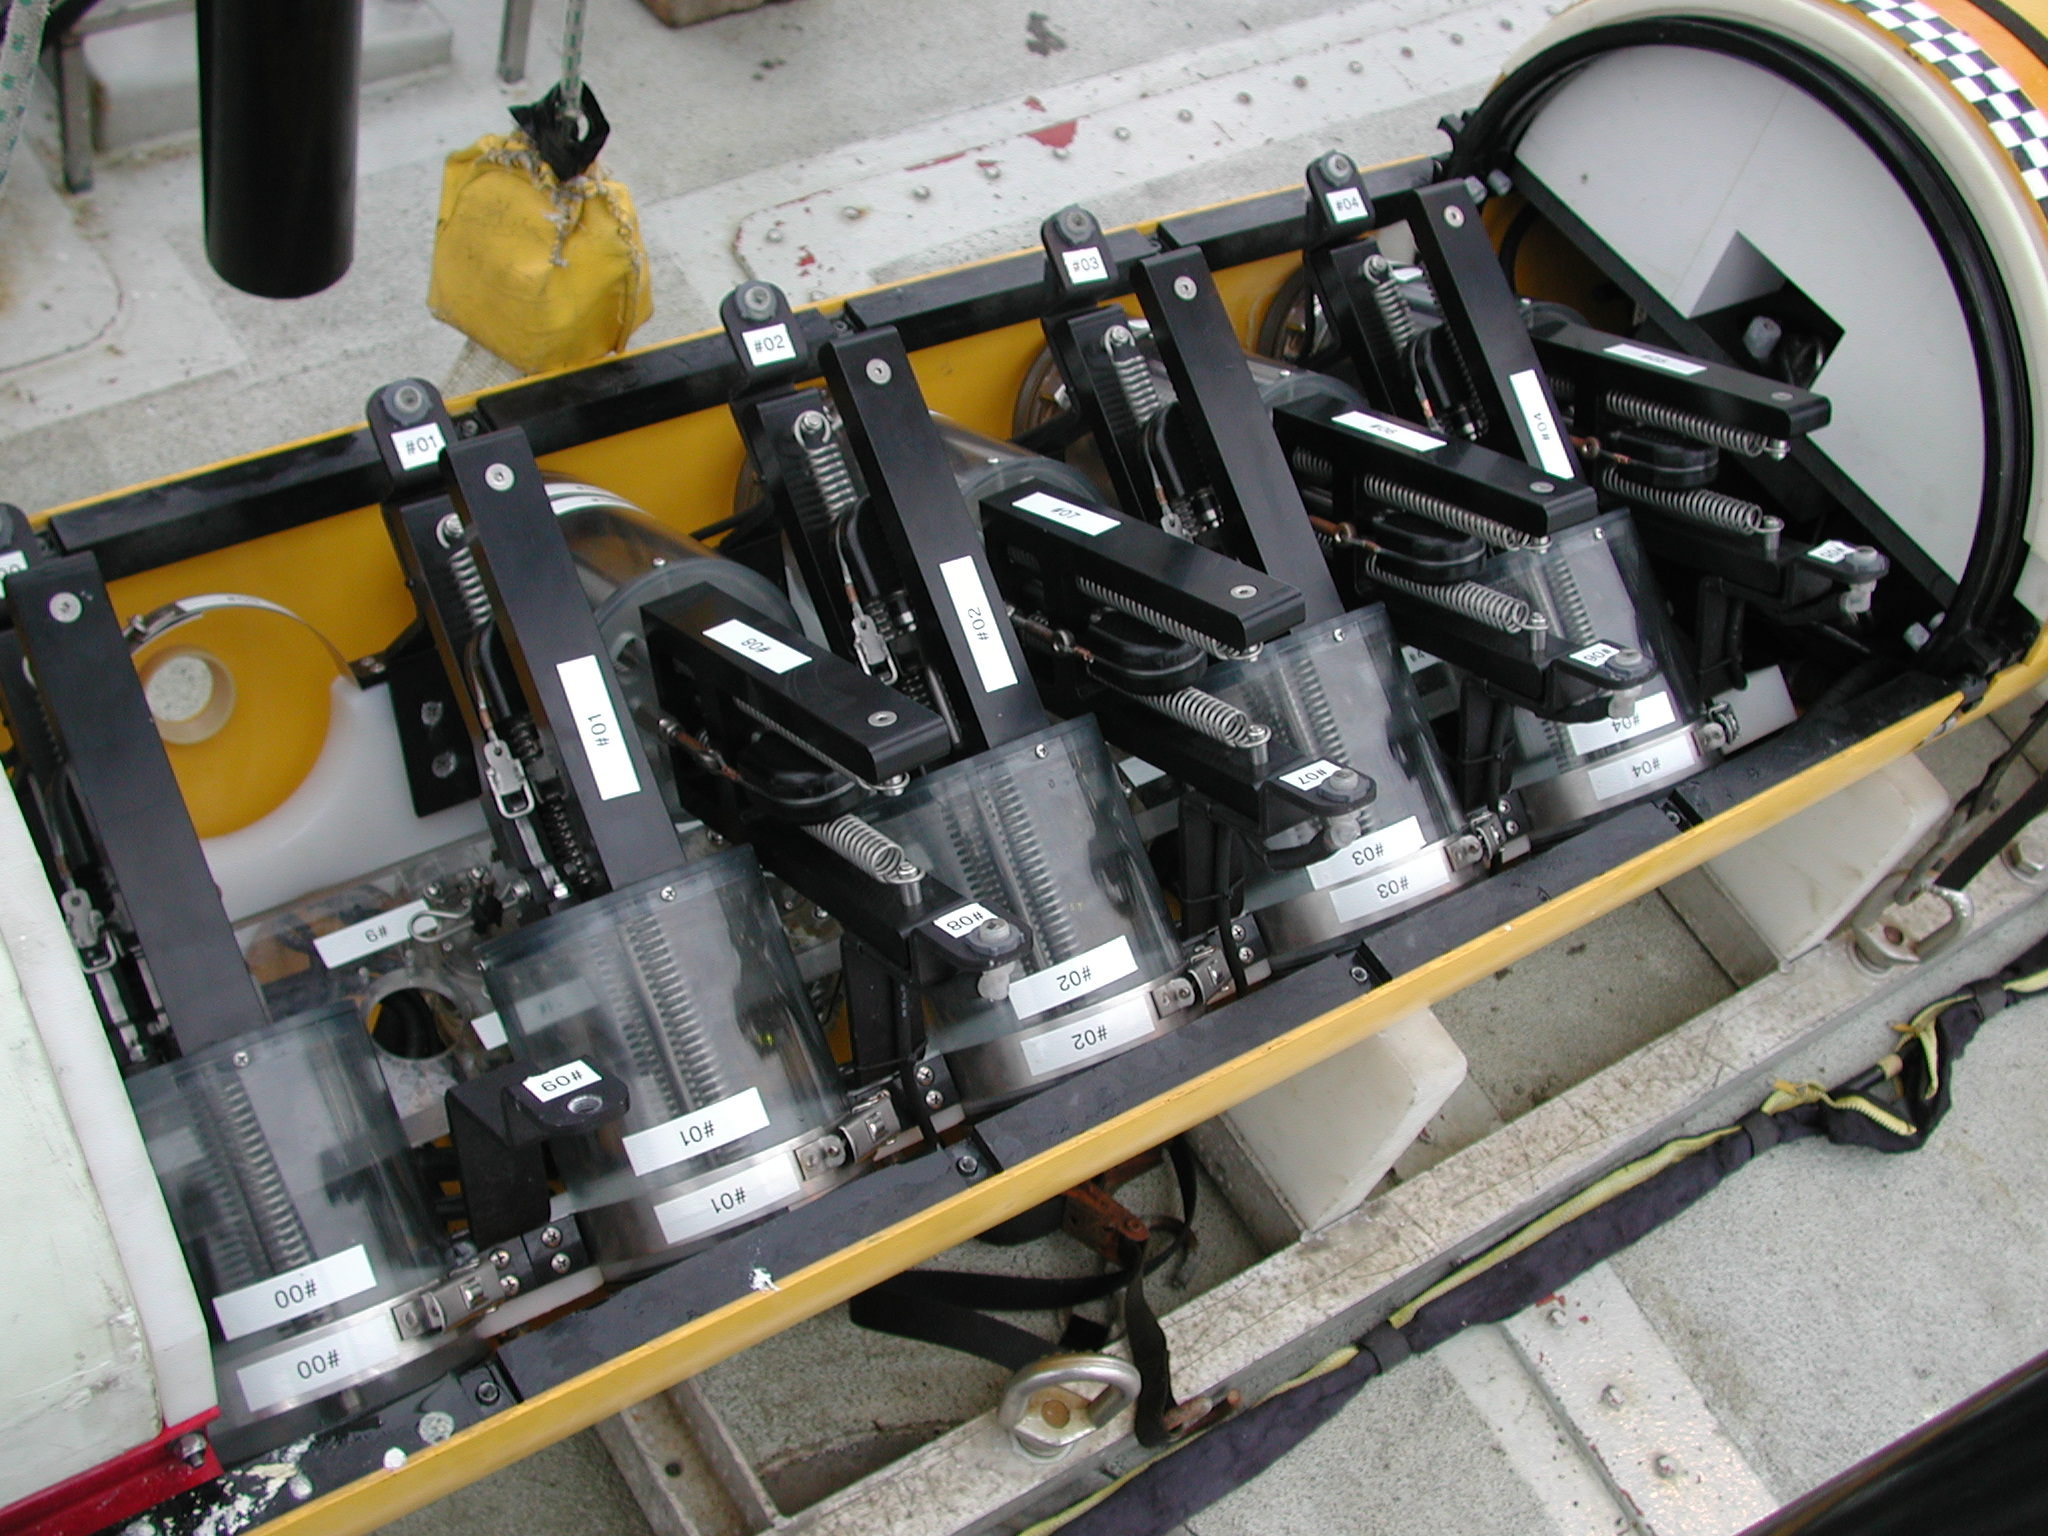
\includegraphics[width=0.35\textwidth]{figs/gulper.jpg}
\caption{\small{The Gulper water sampler \cite{Bird07} on MBARI's
    upper water-column Dorado AUV.}}
\label{fig:gulper}
\end{figure}

A significant driver of the applicability of our work was the
implementation of MBARI's \emph{Gulper} water-samplers \cite{Bird07},
$2$ litre syringe style containers $10$ of which are encased within
the mid-body section of our Dorado vehicle as shown in Fig
\ref{fig:gulper}. However, the original design and intended use of
operation continued to dominated by a naive belief of collecting and
returning water samples as traditional ship-borne methods often
employ, namely using pre-scripted methods, albeit on a highly capable
robot. With the installation of \rx onboard the Dorado with its
capability to synthesize plans and replan on the fly, more imaginative
methods of sample acquisition were targeted.

Our early work focused on observing and sampling within Intermediate
Nephaloid Layers (INLs) \footnote{INLs are fluid sheets of suspended
  particulate matter that originate from the sea floor
  \cite{mcphee-shaw2006}} \cite{ryan10}. The location and scale of
INLs in the water column, which depend upon seasonal and episodic
variability, are not predictable. In turn, they can be identified by
their high turbidity and low chlorophyll fluorescence. Initial
objectives focused on ways to enhance survey results by ensuring as
large a coverage as possible so that INL fields were observed at
tighter spaced transects and when no INL is detected, then transect
spacing in the lawn mower can be incrementally increased. Follow on
work directly targeted sample acquisition within INLs which are often
sparse, patchy in large horizontal scales (in Kms) and small vertical
scales (in meters). Fig. \ref{inl} shows one example from an AUV
transect from 2005. The intent of both observation and sample
acquisition was to interrupt the nominal plan-execution cycle and
inject an action to alter and re-factor the plan dynamically; in one
instance altering the navigation, the other in actuating a sampler.

\begin{figure}[htpb]
\centering
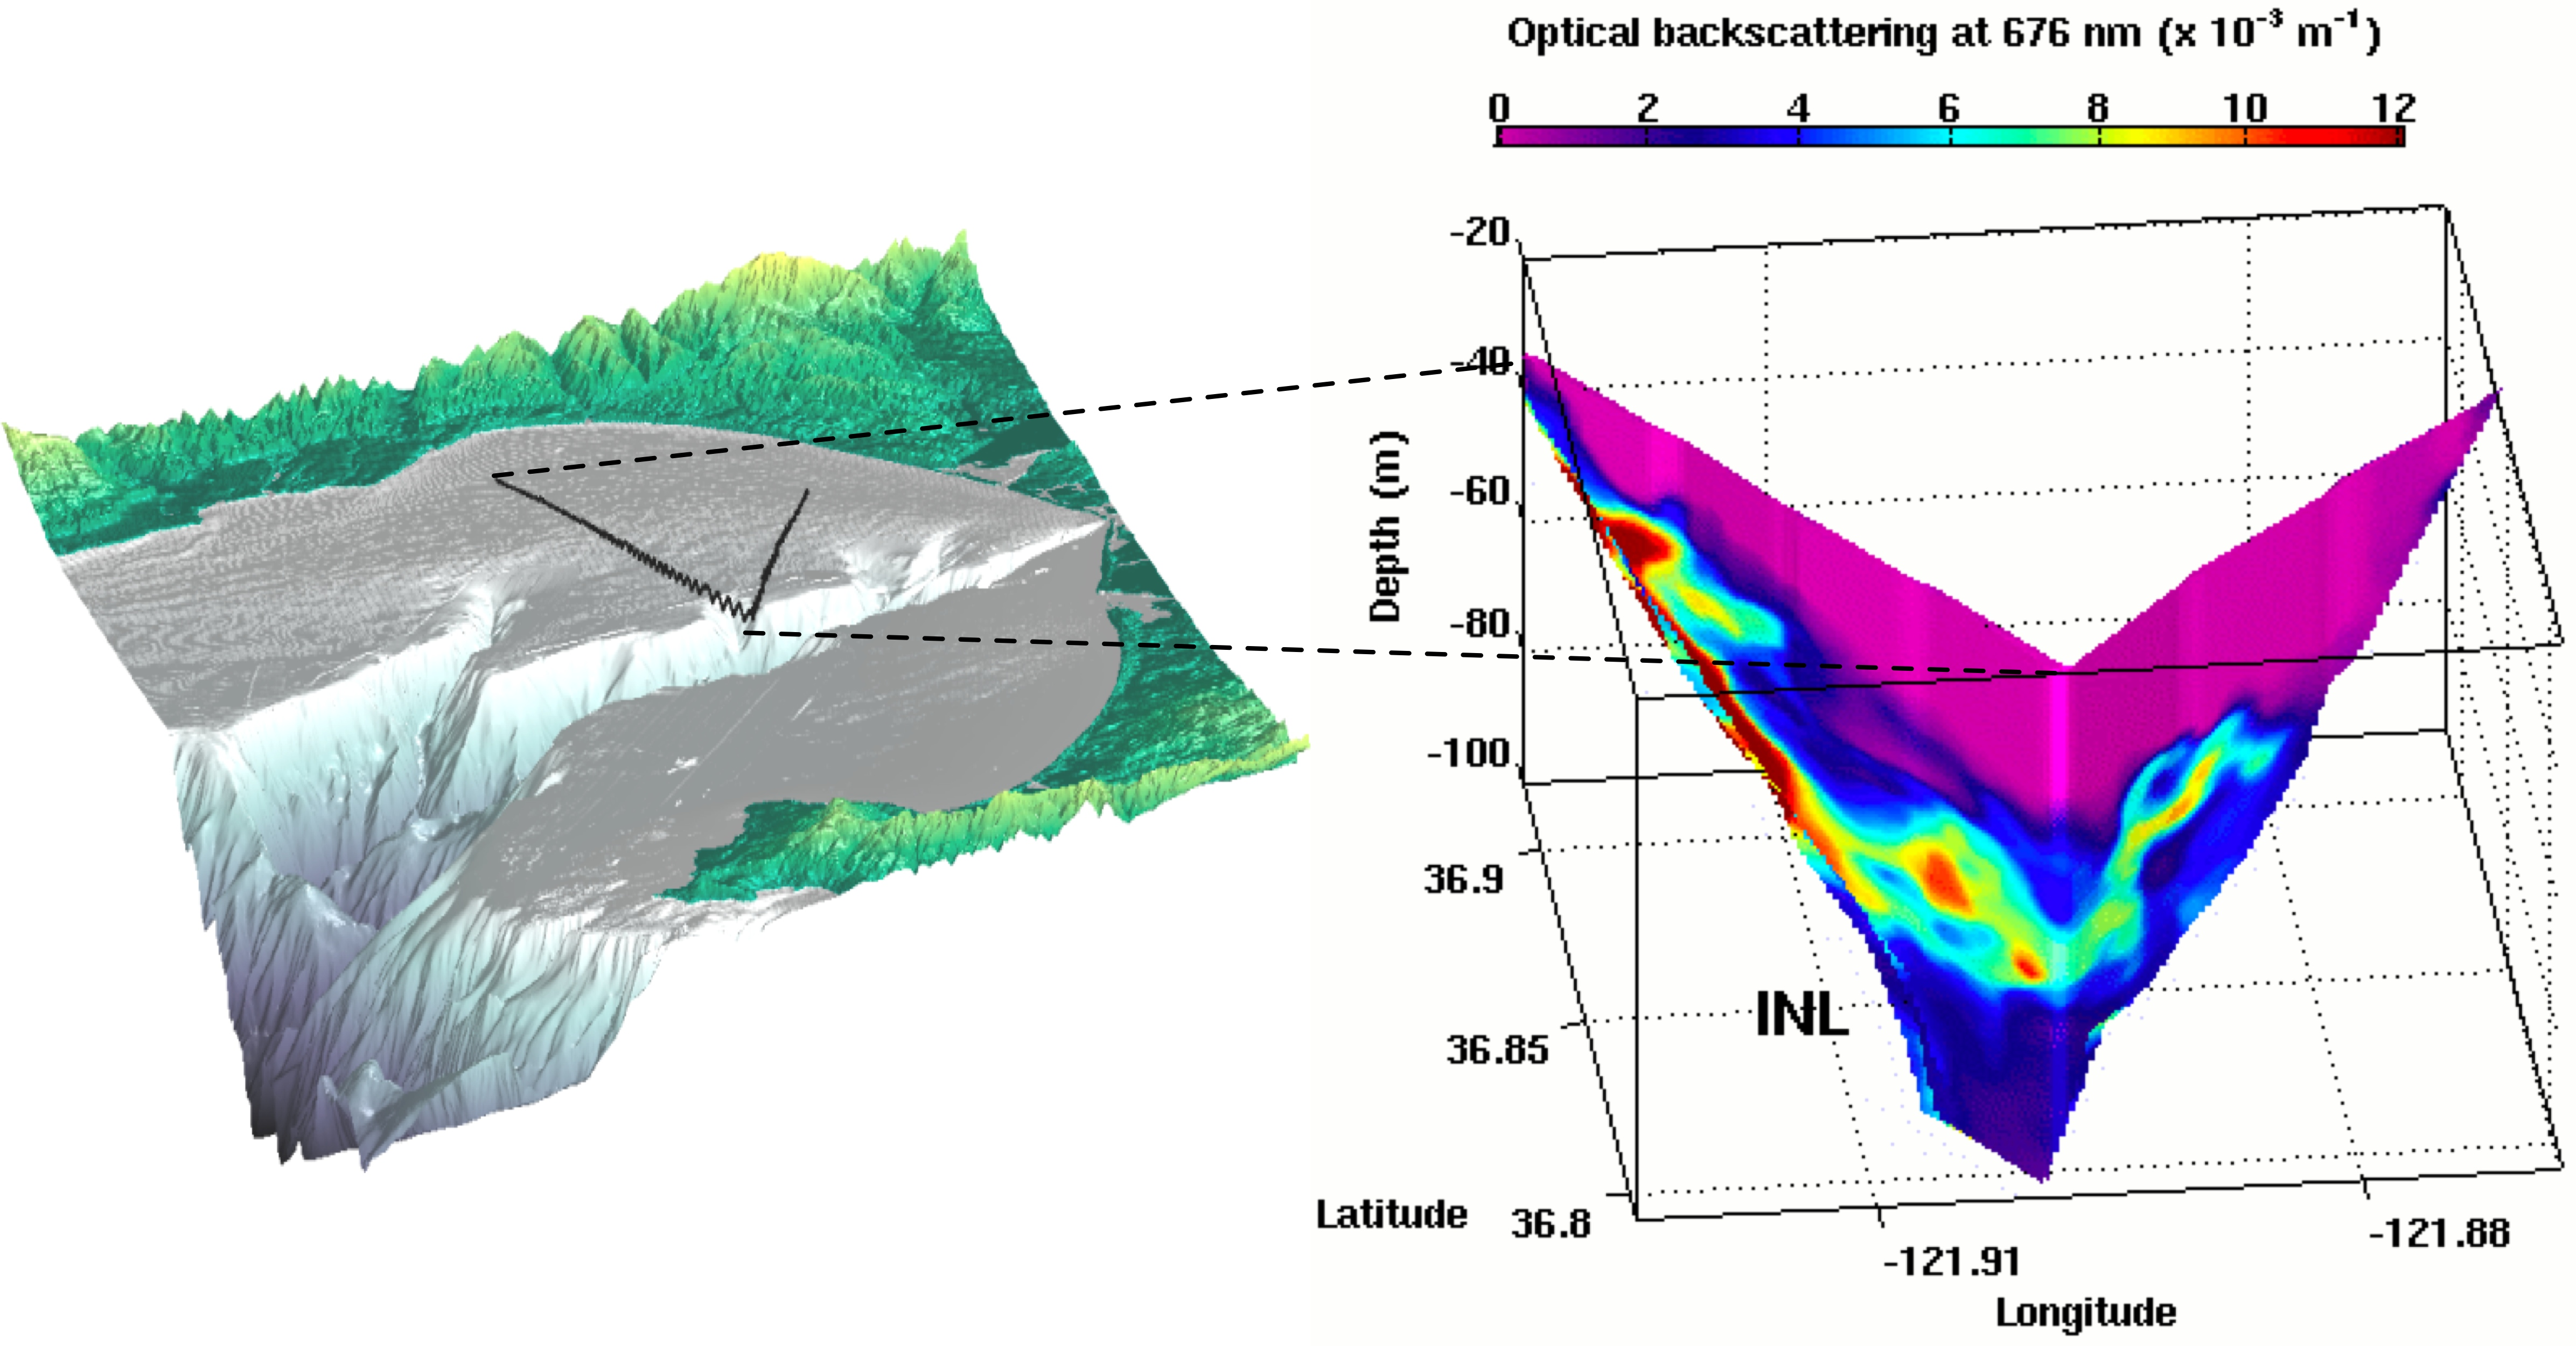
\includegraphics[scale=0.65]{figs/inl.jpg}
\caption{\small An Intermediate Nepheloid Layer (INL) detected by an
  AUV mission in the Monterey Bay in August 2005, showing the location
  of the AUV transect in the bay (left) and optical backscatter image
  at the 420 Nm frequency showing the INLs patchy nature
  (right). \emph{Image courtesy: John Ryan, MBARI}}
\label{fig:inl}
\end{figure}

The implied assumption of installing the samplers on an AUV was that
robotic methods to actuate sample acquisition (with no human control),
would be competitive with human knowledge of where and when to sample
a feature given available shipboard data. To support this assumption,
it required new ways to couple sample acquisition with AUV navigation
and control. While some simple and ad-hoc approaches \cite{yanwu10,
  yanwu11} have shown promise, these techniques were tailored to solve
a specific problem with assumptions on feature structure.  Our
approach on the other hand, stemmed from the need to build a coarse
grained computational model of the INL feature where none existed and
to use that model as a basis to close the \emph{sense-sample-acquire}
loop within the AUV. \cite{fox2007} documents earlier work in using a
well-known unsupervised method in classification the \emph{Kohonen
  Network} or Self-Organizing Maps (SOM) \cite{kohonen} to
\emph{reactively} acquire samples with plan alteration. In doing so we
couple the immediacy of feature identification which is necessarily
reactive, with the deliberation of an onboard temporal planner to
actually trigger a sampler. This has two benefits. First, it goes to
the core of having a deliberative approach to mission planning by
balancing the immediate with that which is projected. Doing so allows
a more systematic approach in dealing with spatial factors in sampling
large volumes. Second, it allows other sampling parameters which are
not directly impacted by perception to be brought to bear; in our
case, scientists would like to introduce constraints (spatial
separation, feature bias, distribution of samples when tracking
multiple features). These are critical not only for science but for
informed decision making which pure reactive approaches simply cannot
undertake.

While the early experiments in \cite{fox2007} coupled the classifier
with the onboard planner, two further novel extensions to sampling
were added. First, to enhance the classifier model by adding a
temporal dimension with a Hidden Markov Model (HMM) \cite{rabiner86,
  Rabiner89atutorial}.  An HMM is a sequential state transition model
in which the current state is not directly visible, but an
observation, dependent on the state, is.  Each state has a probability
distribution over the possible observations.  Therefore the sequence
of observations gives some information about the sequence of traversed
states in the HMM. Unlike identification models based on the simple
classification scheme, HMMs use the dynamics of transition between
modeled states to exploit sequential information of the sensor
readings providing more robust formulation for environmental state
identification. The temporal probabilistic transition then acts as a
filter on top of the clustering model since it is not only derived
from it, but it informs the planner of a potential trigger state only
when the models' transition occurs to an appropriate state of
recognition of the INL feature \cite{mcgann08b}. Not only was
deliberation aided by direct perception of the state (of the INL) but
temporal transition functions added a further level of validation
between expected states in the INL model. This coupling of Machine
Learned model with a deliberative planner is novel in the ocean
sciences and is a continuing direction of investigation \cite{kumar11,
  sergio12}.

The second innovation involved dynamic resource allocation associated
with the water samplers \cite{olaya11}. Using a priori sample
utilities coupled with temporal and spatial information maintained by
the deliberating planner in-situ, the algorithm dynamically generates
a policy on sample acquisition during the course of the mission. In so
doing, utility functions can be used to balance sparcity or abundance
of the feature encountered with the availability of samplers
dynamically. Coupled with periodic sub-sampled science data returned
by the vehicle when on the surface and goal-oriented commanding with
\rx, such a capability allows judicious use of the limited samplers by
a scientist from her desktop.


\paragraph {Mixed-Initiative Frontal Tracking:} We exploit the
in situ decision making capability of \rx in order to find and
continuously map a thermal gradient. The strategy encapsulated in
algorithms onboard is described by the following three phases:

\begin{figure}[htpb]
\centering
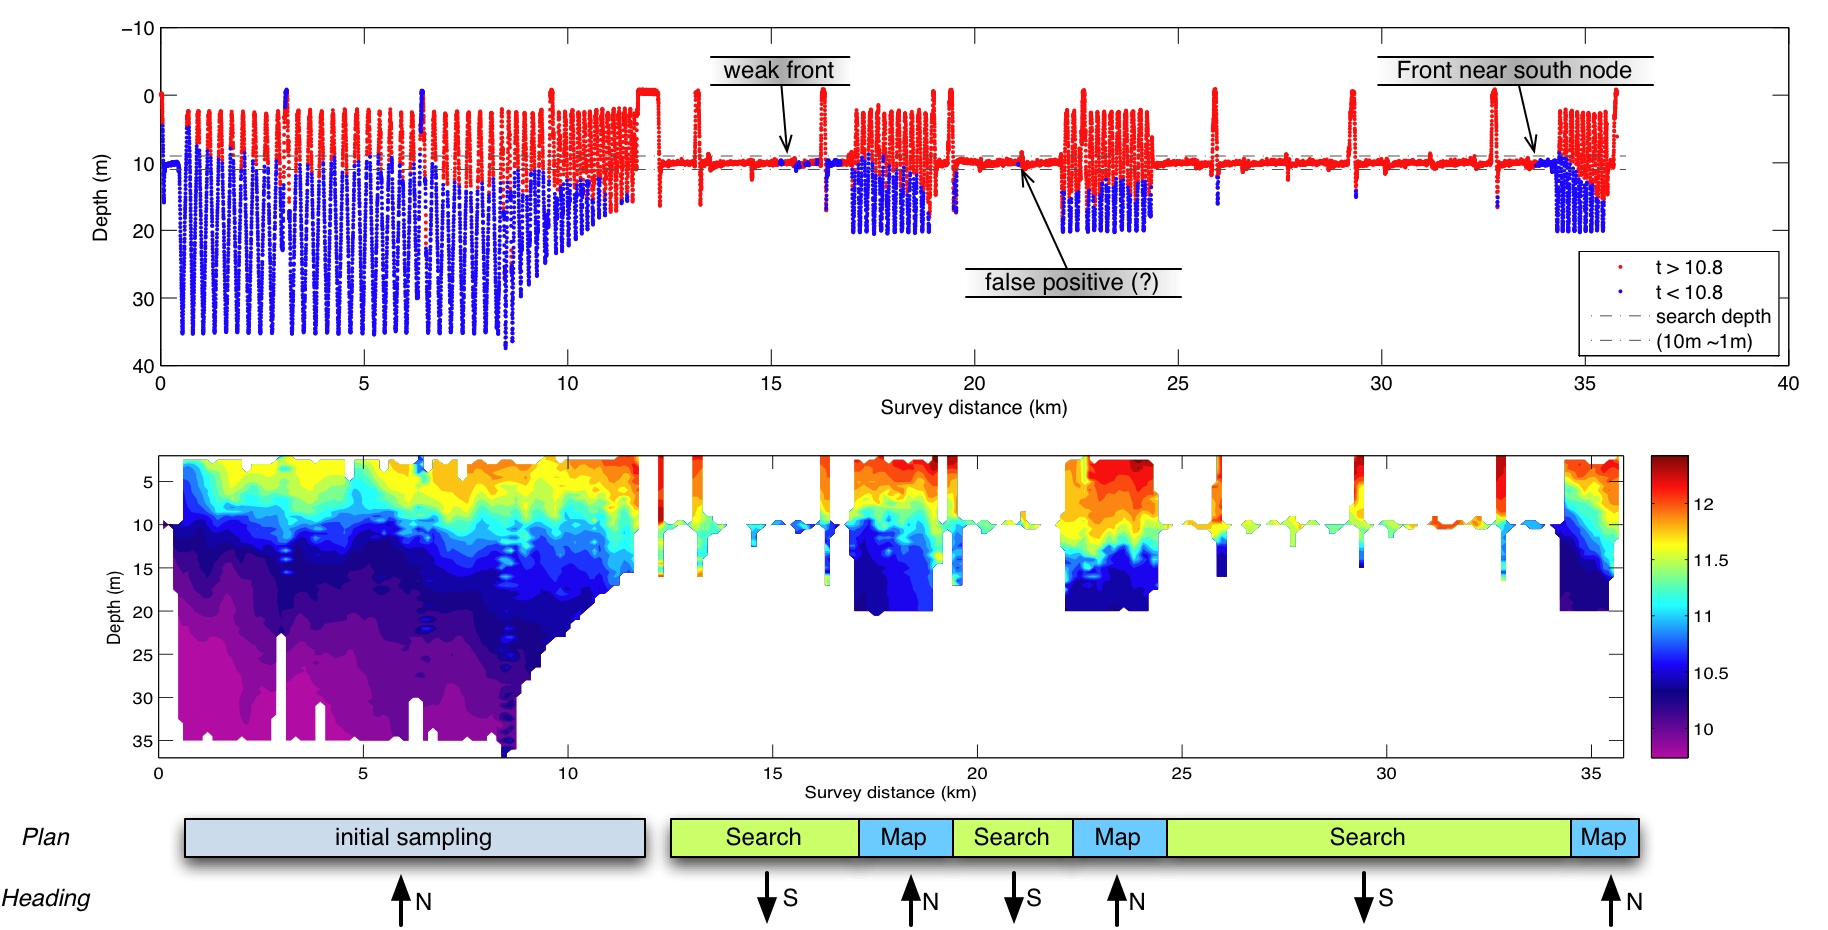
\includegraphics[width=0.8\textwidth]{figs/front-mi.jpg}
\caption{\small{Survey trackline of AUV following a thermal
    gradient. Image in the middle shows the temperature while the
    bottom figure shows different phases in the algorithm.}}
\label{fig:mi-front}
\end{figure}

\emph{Mapping}: The vehicle performs a yo-yo transect between two
designated waypoints and sends temperature sampled every $5$ meters to
shore via satellite. The temperature field is reconstructed from
interpolation of the transmitted data, and the scientist identifies
the target front. Using a graphical user interface, she is then able
to generate a high-level command which represents the front as a
temperature threshold ($t^{\circ}$) at a given depth ($d$). This goal is
then appropriately packaged and sent to the AUV via satellite.

\emph{Search}: After the mapping phase and on receipt of this message
on the vehicle T-REX evaluates the goal, automatically synthesizes a
set of waypoints by generating a plan and then dispatches the plan to
execute by having the vehicle swim back and forth at depth $d$ all the
while reactively evaluating when a temperature threshold $t^{\circ}$
is crossed. In the process \rx checks both the depth and temperature
sensed by the AUV; when the depth is around $d$ ($\pm 1$ meter to
account for vehicle control uncertainty), it then compares the
temperature read with $t^{\circ}$. When the comparison value changes \rx
assumes that the front is identified and switches into the next phase.

\emph{Sampling}: The vehicle undertakes a small transect around the
identified front location while actuating water samplers, one at the
center of the front with temperature threshold $t^{\circ}$, and one on
either side of the front. When this transect is completed, \rx
switches back to the Search phase to follow the frontal evolution.
The survey is completed either when we reach the maximum mission
duration or the vehicle returns to its initial waypoint during the
search phase without crossing the threshold $t^{\circ}$. The latter is
indicative of the frontal zone having left the survey domain.

The novelty in this application was two-fold; in enabling the
deliberation to decide when to decide on the phase changes and in
showing viably how a human being coupled with a goal-oriented
controller could do problem solving jointly. The approach, is general
and can be adapted to any feature or scalar field.

\paragraph {Lagrangian Surveys:} More recent experiments with \rx
controlling the Dorado AUV have centered on the \texttt{CANON}
(Controlled, Agile, and Novel Observing Network) program at MBARI. The
fundamental science goals of the program are related to detecting and
tracking of spatio-temporal coastal ocean features \cite{canon}. The
dynamic features require a robotic platform to move with it, return
water samples from across and within gradients and provide contextual
observations to other drifting instruments. All of these observational
strategies are tied to vehicle adaptation which is intrinsically tied
to deliberation and difficult to accomplish otherwise.

Various adaptation methodologies in \texttt{CANON} are still being
investigated; however what has become a critical goal for the program
has been to provide contextual environmental information about water
patches. The form and content of such 'patches' varies; for instance
initial attempts focused on Harmful Algal Blooms (HABs). They have
large spatial ($>$ 50 km$^2$) and temporal (days to weeks) extent and
are visible from space with visible coloring on the ocean surface. The
direct impact of HABs is the introduction of toxins into the marine
(and as a consequence human) food chain. In addition,
\cite{anderson00} and \cite{hoagland06} estimate that the average
economic impact resulting from HABs in the United States has been
$\sim$\$75 million from 1987 to 2000. However, the processes behind
bloom initiation, evolution and collapse is poorly understood in part
due to the complex interactions between microbial communities and the
surrounding environment. As a result, our capacity to assess the range
of potential future scenarios that might result from ocean temperature
changes, acidification, or nutrient shifts is highly limited.

\begin{figure}[htpb]
\centering
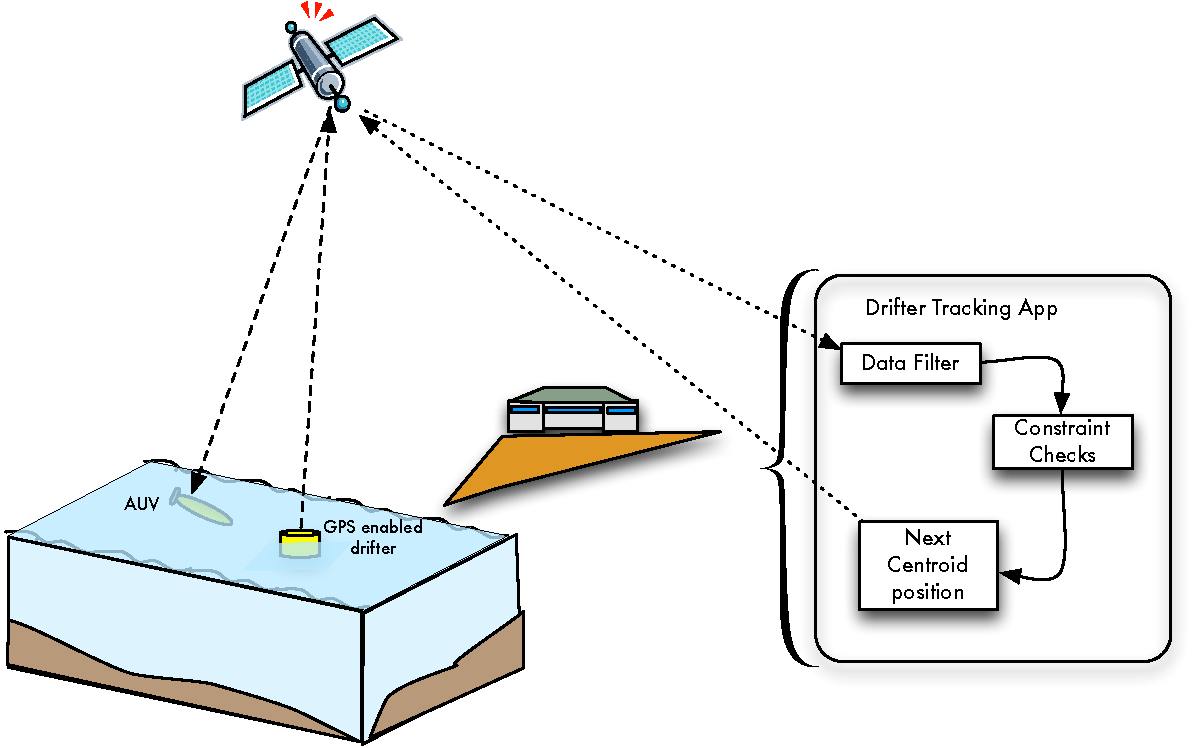
\includegraphics[width=0.5\textwidth]{figs/dta-app.pdf}
\caption{\small{Overall setup of CANON lagrangian experiments with a
    drifting instrument pack. Various combinations of computational
    methods can be included in the Drifter Tracking App which is a
    part of the Oceanographic Decision Support System (ODSS)
    \cite{das11}.}}
\label{fig:dta-setup}
\end{figure}

To augment our understanding of such microbial communities, the Dorado
with \rx has been utilized in a range of activities in a
quasi-lagrangian mode. As the water mass is being tracked with a
drifting instrument, the vehicle is expected to move around it. While
a number of different patterns have been tested in simulation, the
majority of at-sea deployments have used a square pattern ($3X3$
km\textsuperscript{2} or a $1X1$ km\textsuperscript{2})\footnote{Often
  post-hoc reconstruction of the data set for visualization drives how
  much adaptation the vehicle can be allowed to undertake.}. Plan
synthesis occurs frequently, but within the context of a drifting
point generated by a drifter. Fig. \ref{fig:dta-setup} shows the
general setup of our experiments which can be tailored with the use of
various computational methods within the \texttt{DTA} app which is
contained within the Oceanographic Decision Support System (ODSS; see
below) \cite{das11}. GPS data from the free-floating drifter is sent
via satellite and processed onshore to determine a projection (speed
and bearing) of the drifter. This data is sent to the AUV; at the
completion of the current survey, the vehicle receives this data as a
high-level goal which is decomposed and synthesized as a survey
plan. Currently, the vehicle completes the survey without any further
dynamic updates from the drifter. In order to minimize the range of
errors that the survey needs to encapsulate (data latency or surface
or sub-surface currents for those drifters which have a drogue) the
estimation is a projection in time and space of the drifters centroid
sent with this goal from the shore-side app.

\begin{figure}[htpb]
\centering
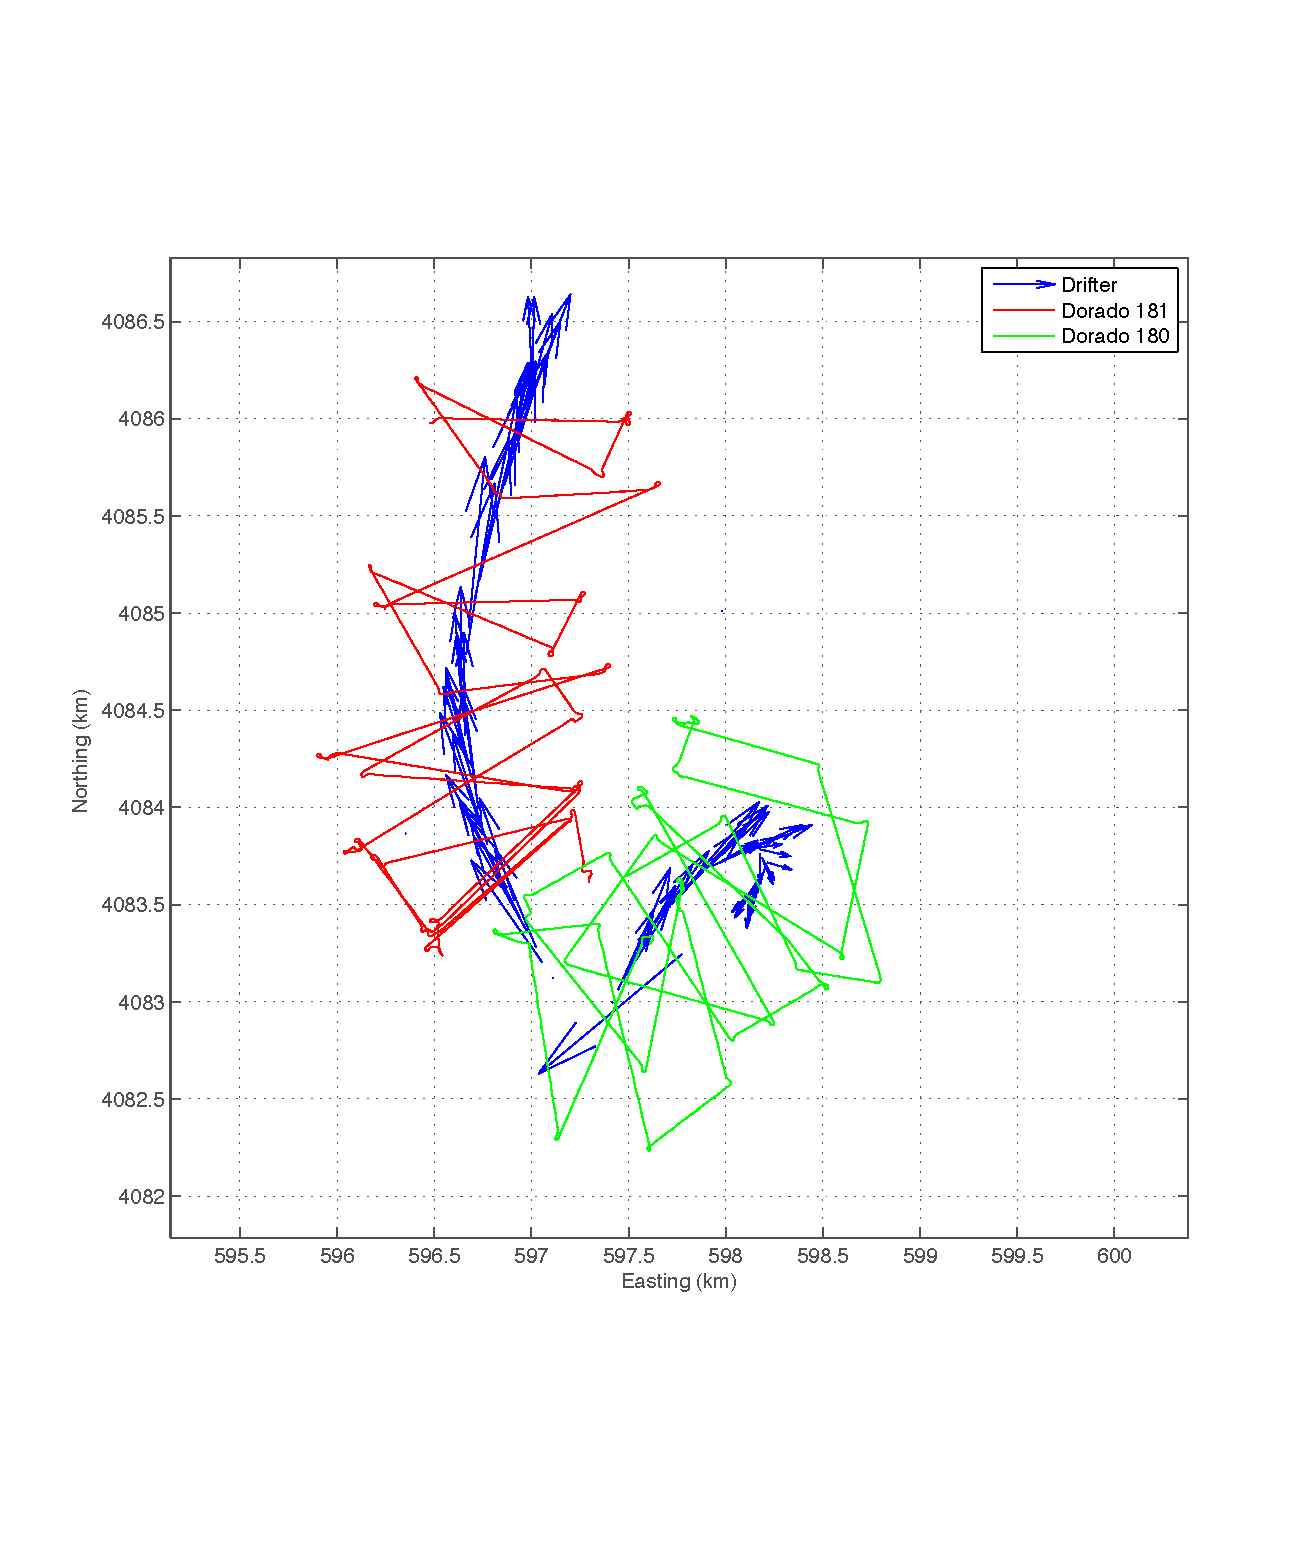
\includegraphics[width=0.35\textwidth]{figs/june11-drifter-follow-180-181.pdf}
\caption{\small{A June 2011 drifter cruise shown in the Earth
    frame. Deviations in the AUV transect are based on the frame of
    reference in addition to positional errors \cite{das11b}.}}
\label{fig:drifter-errors}
\end{figure}

Typically this has meant that the vehicle computes a set of waypoints
for the survey plan, moves to the start waypoint and then executes the
survey even as the centroid is moving. Positional error of the vehicle
and uncertainty in the speed and bearing of the vehicle\footnote{In
  our September 2010 experiment as the drifter moved over the Davidson
  Seamount \cite{clague10} deviation in the California current
  resulted in visible directional change that can be seen in
  Fig. \ref{fig:sep10-transects} at the end of the mission.} exist;
however, the observations of the survey to retain the environmental
context require a change in reference frames so that the patch-center
tagged by a GPS-tracked drifter remains within the survey perimeter at
all times \cite{das11b}.

\begin{figure*}
\centering
\subfloat[]{\label{fig:sep10-ship}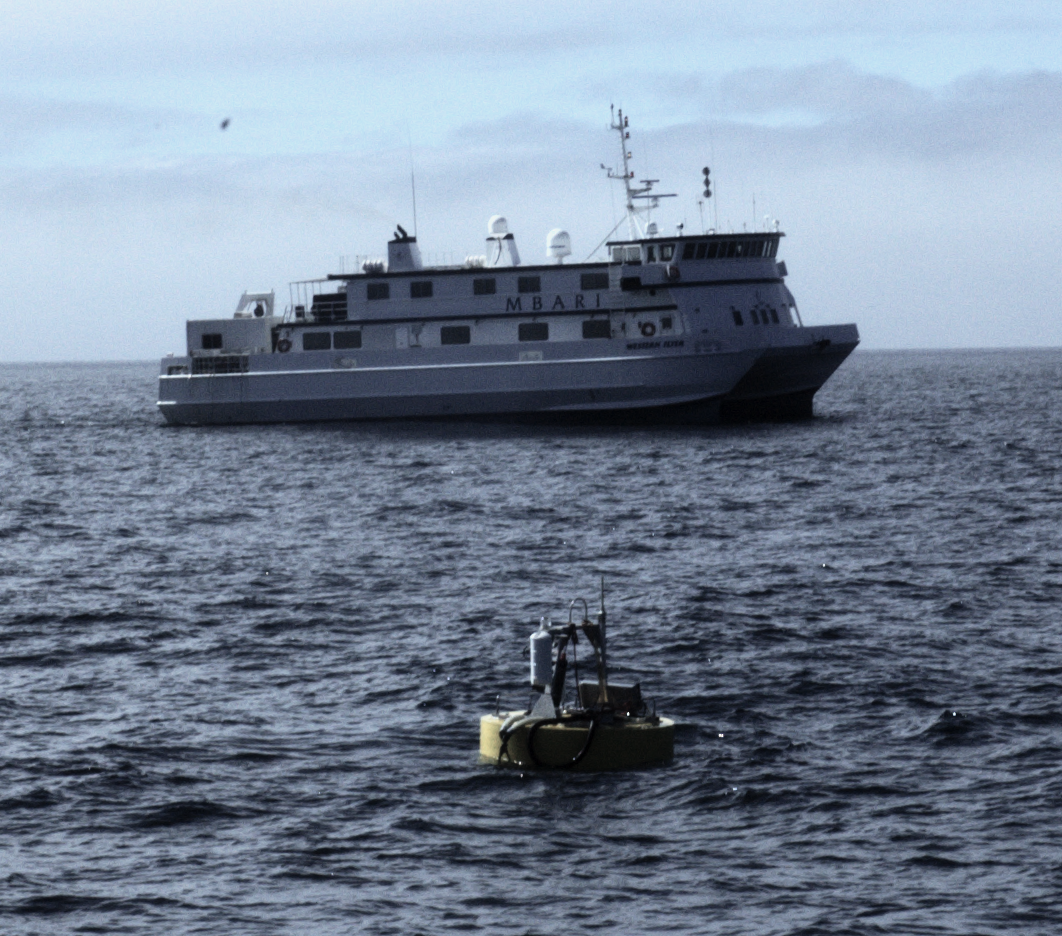
\includegraphics[width=0.38\textwidth]{figs/sep10-canon-cruise.png}}
\subfloat[]{\label{fig:sep10-transects}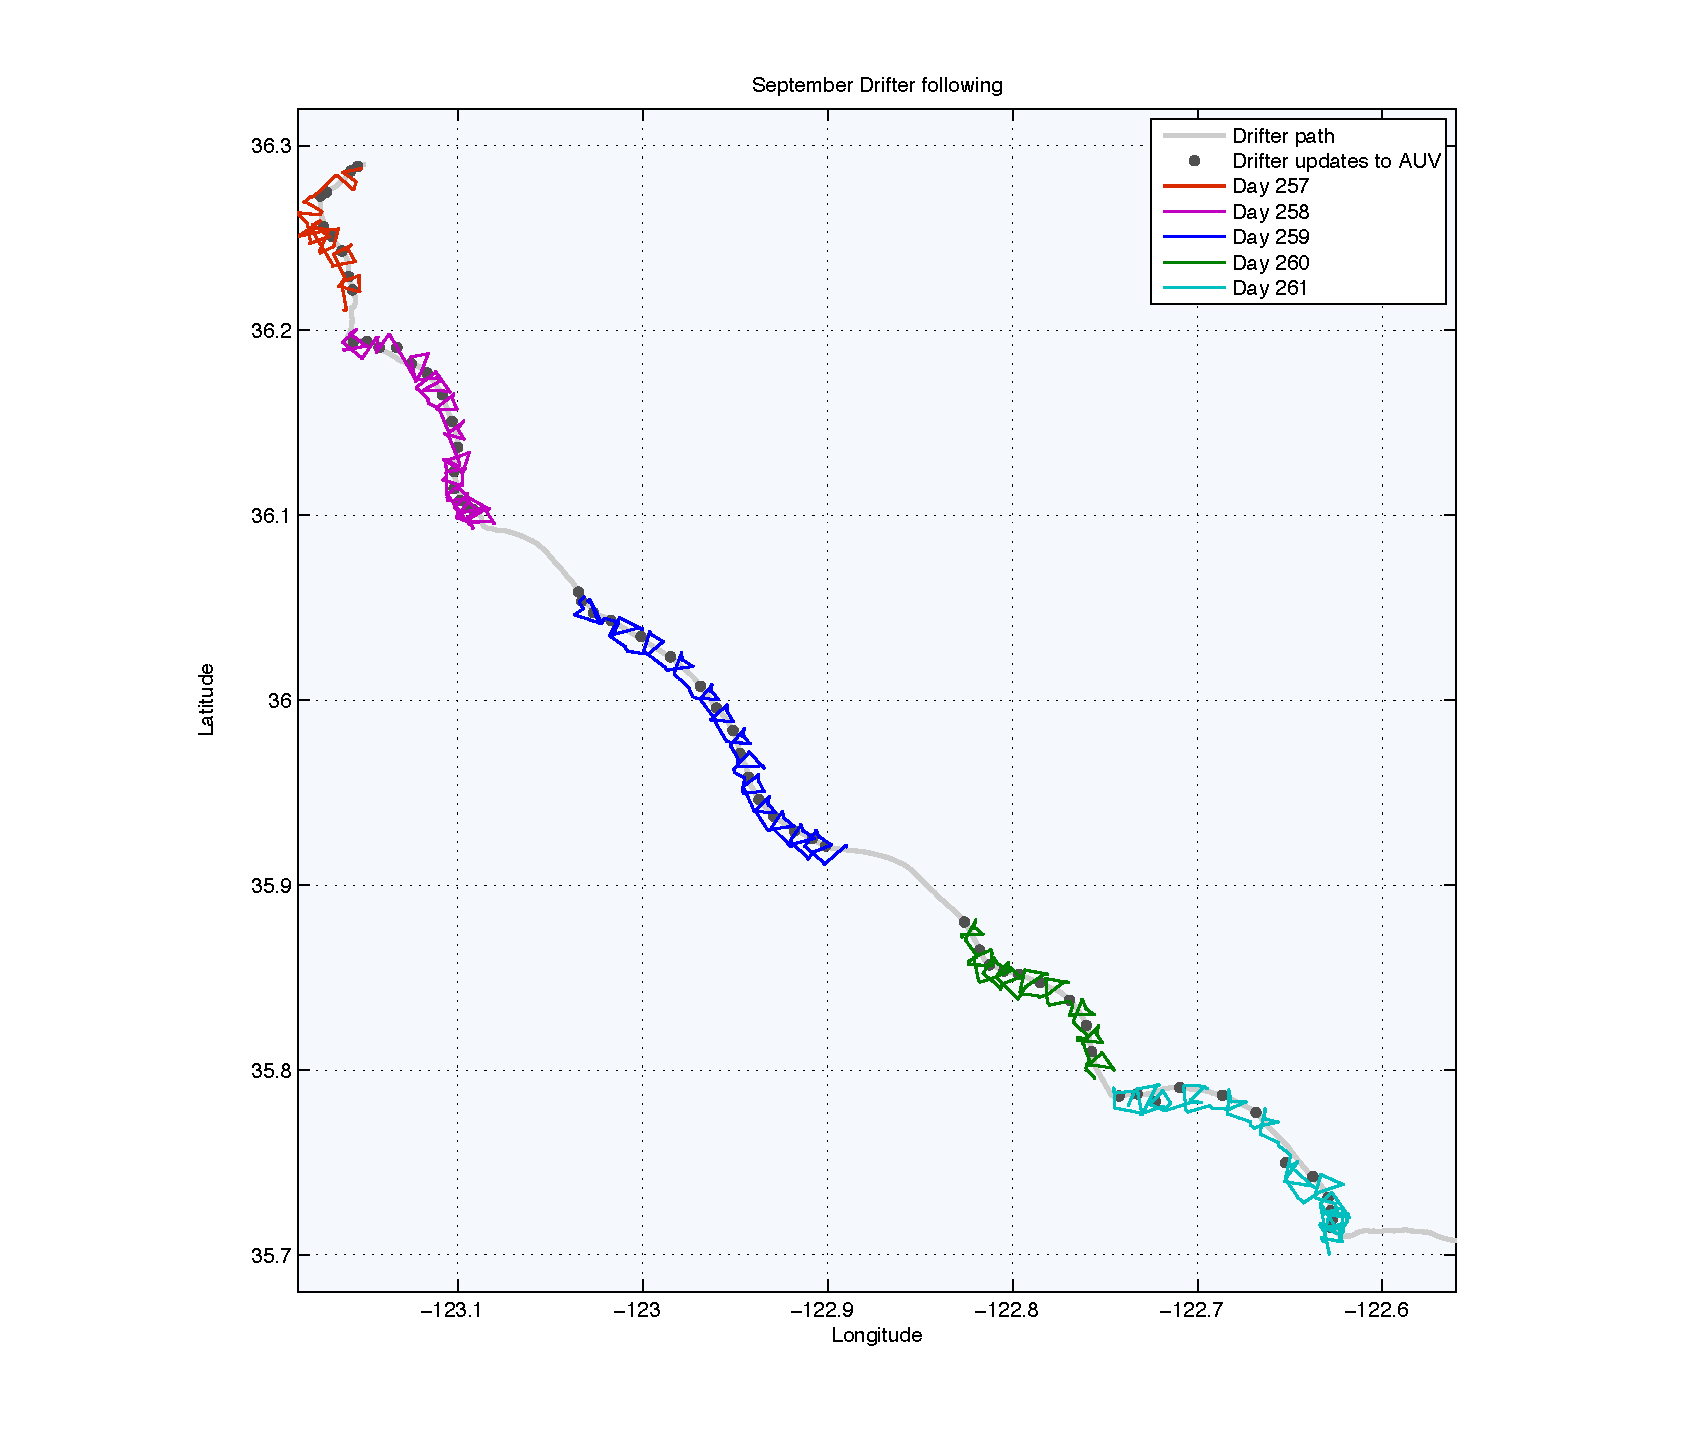
\includegraphics[width=0.35\textwidth]{figs/september-iterations.pdf}}
  \caption{\small{The offshore CANON ESP-drifter following cruise
      \cite{das11b}. Fig. \ref{fig:sep10-ship} shows the ESP drifter
      foreground with the R/V \emph{Western Flyer} with the image
      taken from the R/V \emph{Zephyr}. Fig \ref{fig:sep10-transects}
      shows the 86 km transect of the Dorado following the ESP drifter
      about 100 Nm from California shores.}}
\label{fig:gulper}
\end{figure*}

These theoretic results were validated in a five-day long off-shore
deployment carried out in September 2010, 160 kms off the California
coast (Fig.~\ref{fig:sep10-ship}). A specialized drifter with a
genomic sensor \cite{scholin09} hanging $20$ m below, performing
in-situ identification of micro-organisms was the target. The
experiment was supported by crews on two support vessels, the R/V
\emph{Western Flyer} and the R/V \emph{Zephyr}. The \emph{Flyer}
visited the drifter every four hours to carry out a series of
ship-based sampling experiments and lab analysis on water samples to
ground-truth the drifter sensor data. The \emph{Zephyr} was meanwhile
focused on Lagrangian observation studies using the Dorado with the
goal to monitor the nutrient budget at the perimeter of a $1$km $X
1$km water patch around the advecting drifter while the AUV performed
a transformed box pattern around the drifter. A number of logistical
issues were kept in mind while designing and executing the
experiment. Each iteration began with the latest drifter update
(position and velocity) received from the drifter through a satellite
link which was transmitted to the vehicle for in-situ adaptation. \rx
used this input to compute the $5$ waypoints necessary for an
iteration of the box pattern, with the AUV traveling at constant
velocity in the earth frame. Waypoints were computed once at the
beginning of the survey with the AUV surfacing once for every survey,
with each survey lasting $\sim1$ to $1.5$ hours. A total of 60 surveys
were attempted over the course of the $5$
days. Fig. \ref{fig:sep10-transects} shows the overall transects over
the course of the mission, with gaps in between days when the AUV was
being recharged. Each deployment lasted $\sim12$ hours. The black dots
in the figure show the beginning of each iteration when drifter
updates were received by the AUV.


\begin{figure}[htpb]
\centering
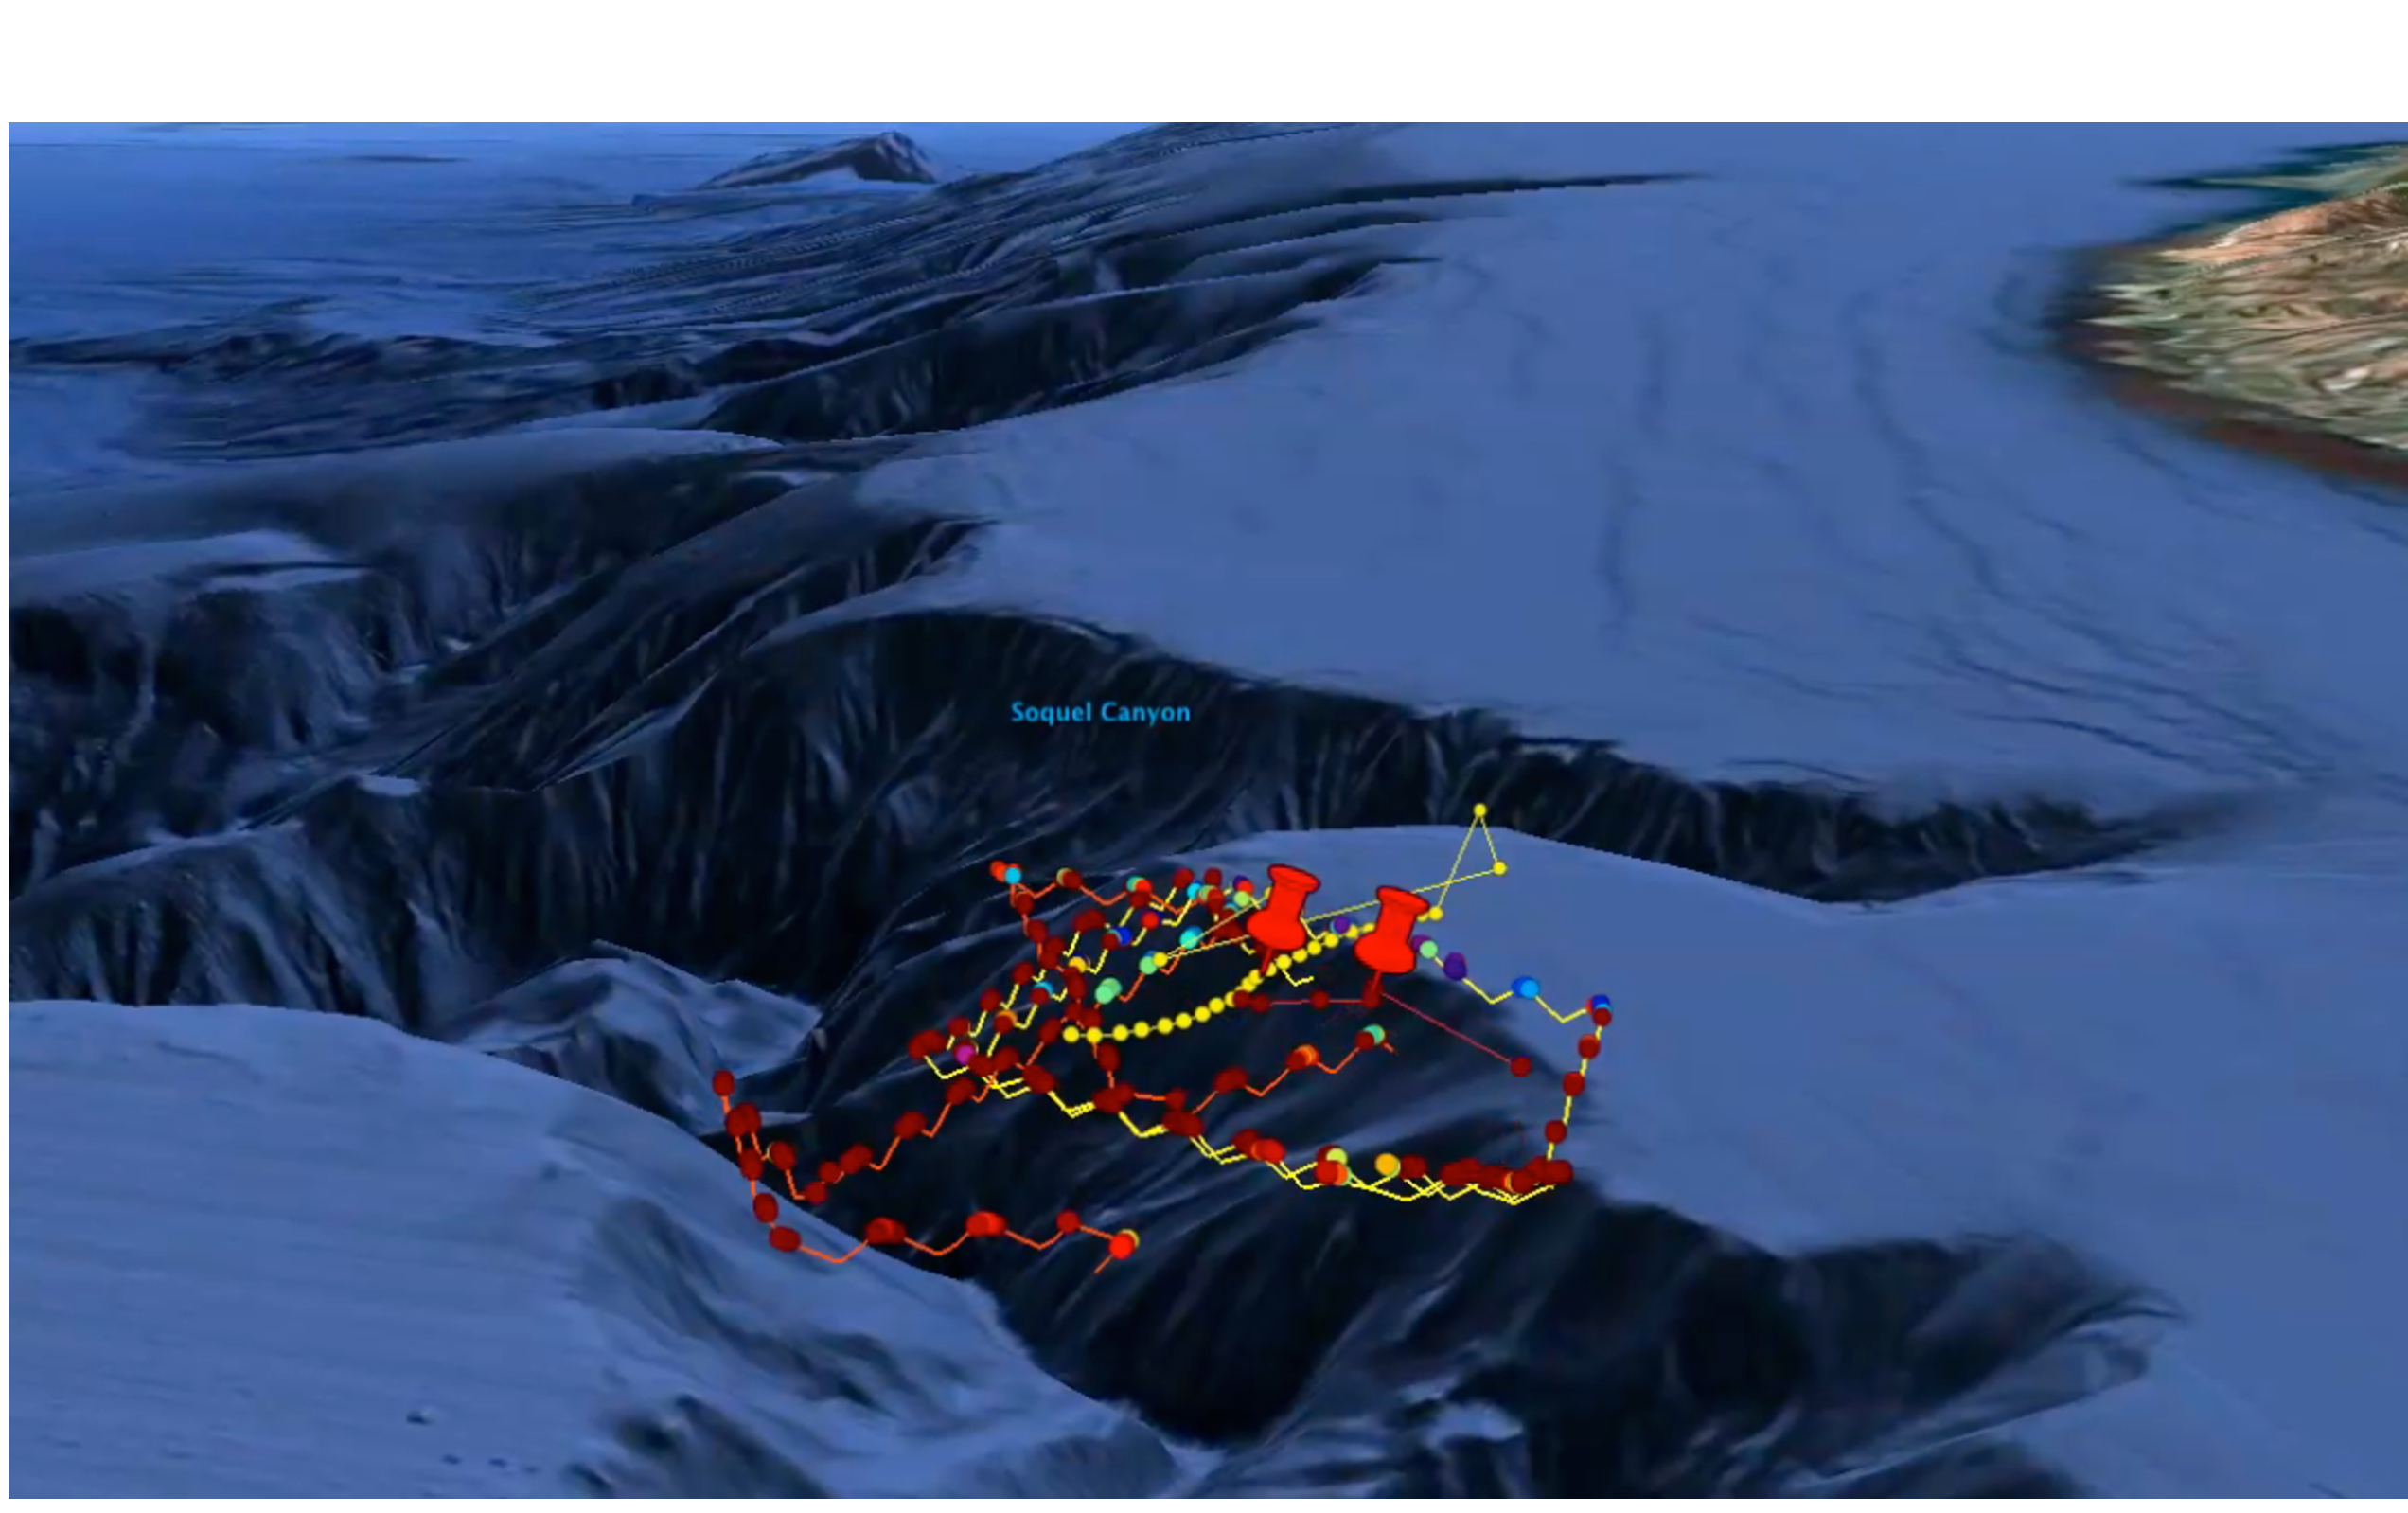
\includegraphics[width=0.7\textwidth]{figs/oct10-ballet.pdf}
\caption{\small An October 2010 robot ``ballet'' where a smaller
  slower AUV tracked a patch center, sending periodic updates to the
  Dorado using a setup shown in Fig. \ref{fig:dta-setup}. The Google
  Earth post-hoc image shows red track lines of the \rx commanded
  Dorado with the yellow transects of the LRAUV. Yellow dots show the
  track line of a simple GPS-enabled drifter used for seeding the
  experiment over the Monterey Canyon with Santa Cruz, CA to the right
  of the figure.}
\label{fig:ballet}
\end{figure}

Successive lagrangian experiments also followed a more innovative and
robotically choreographed ``ballet'' between two AUVs, the Dorado and
the LRAUV \cite{bellingham10} in October 2010 as part of another
series of \texttt{CANON} field experiments. The slower vehicle with a
fluorometer tracked a targeted chlorophyll patch seeded by a
GPS-enabled drifter, sending periodic updates of the patch centroid to
shore via the ODSS following a setup similar to
Fig.\ref{fig:dta-setup}, to the Dorado running \rx. 

\begin{figure*}
\centering 
\subfloat[Temperature]{\label{fig:sep11-temp}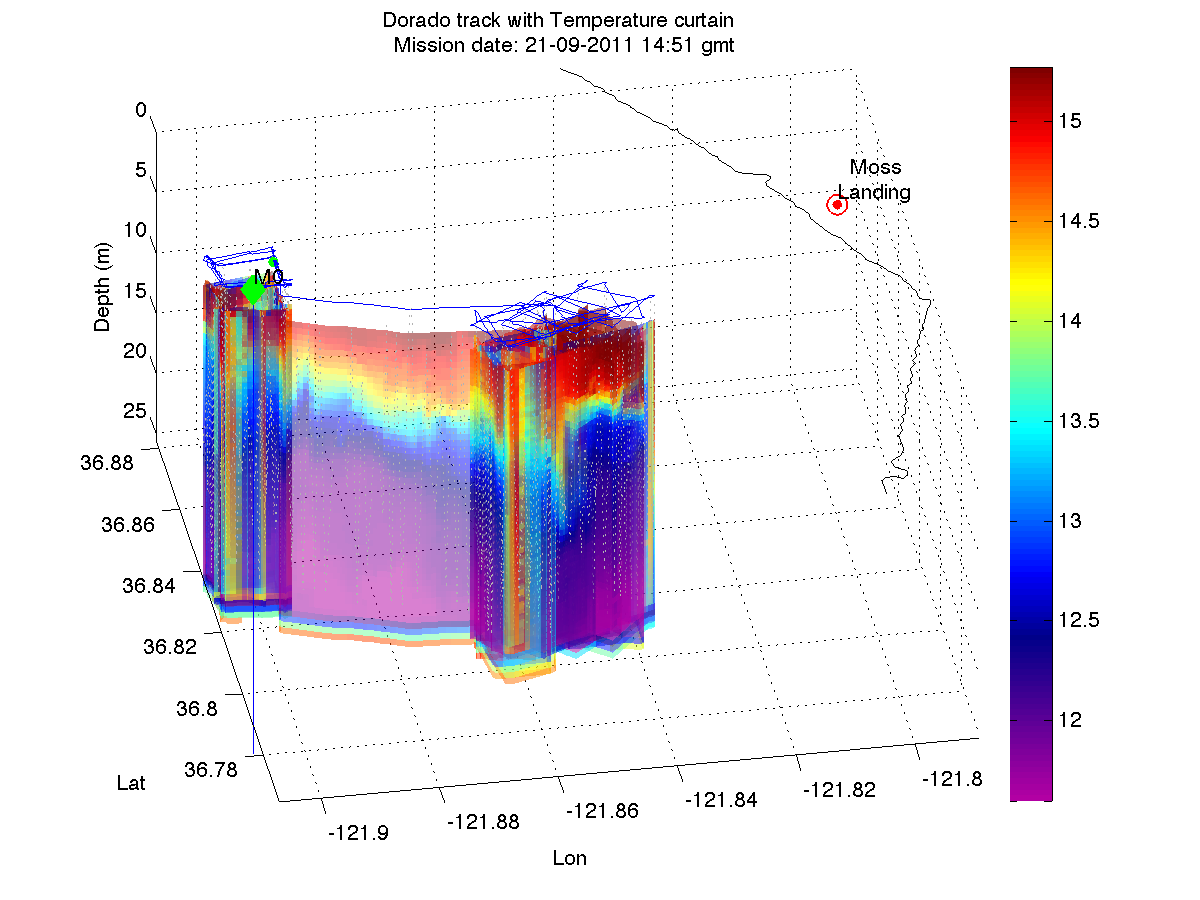
\includegraphics[width=0.5\textwidth]{figs/sep11-ww-temp.png}} 
\subfloat[Salinity]{\label{fig:sep11-sal}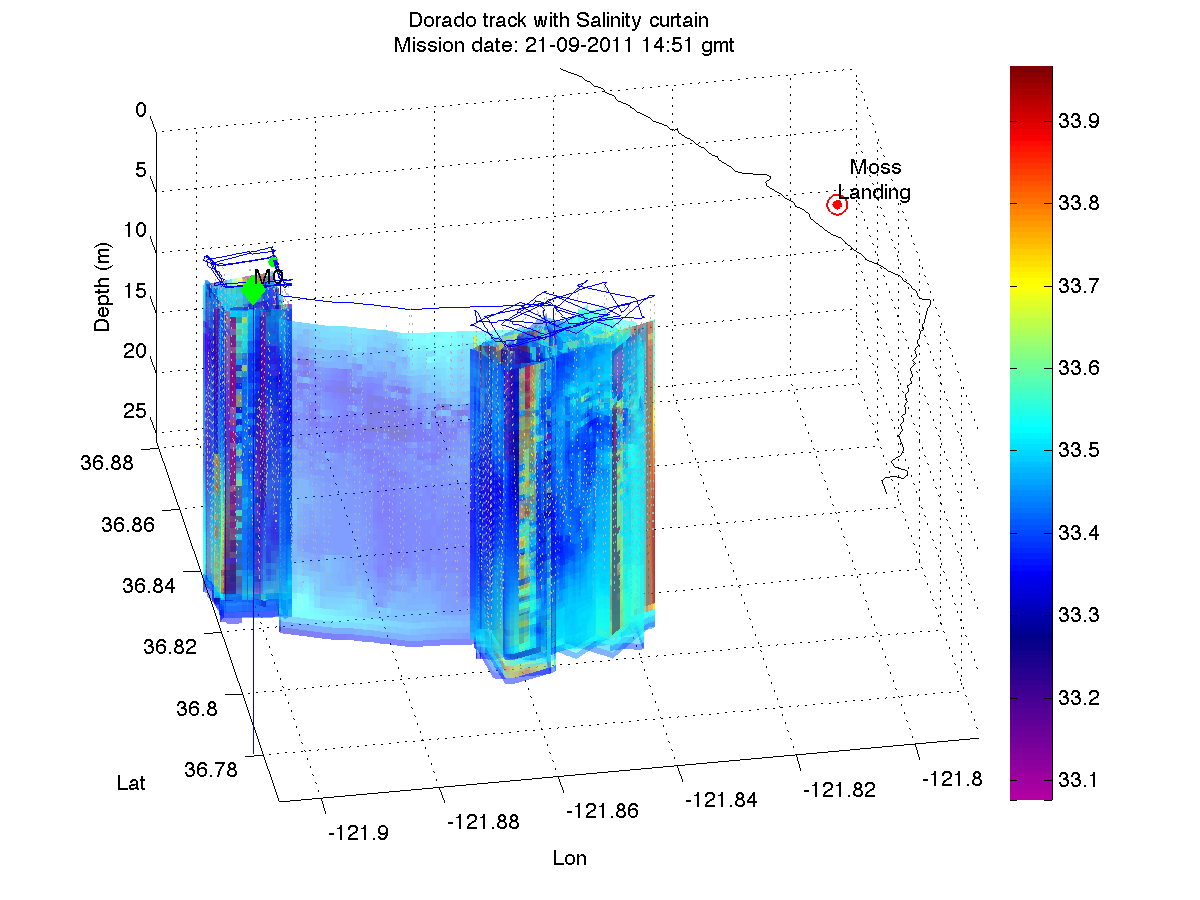
\includegraphics[width=0.5\textwidth]{figs/sep11-ww-salinity.png}}\\
\subfloat[Fluorescence line height]{\label{fig:sep11-flh}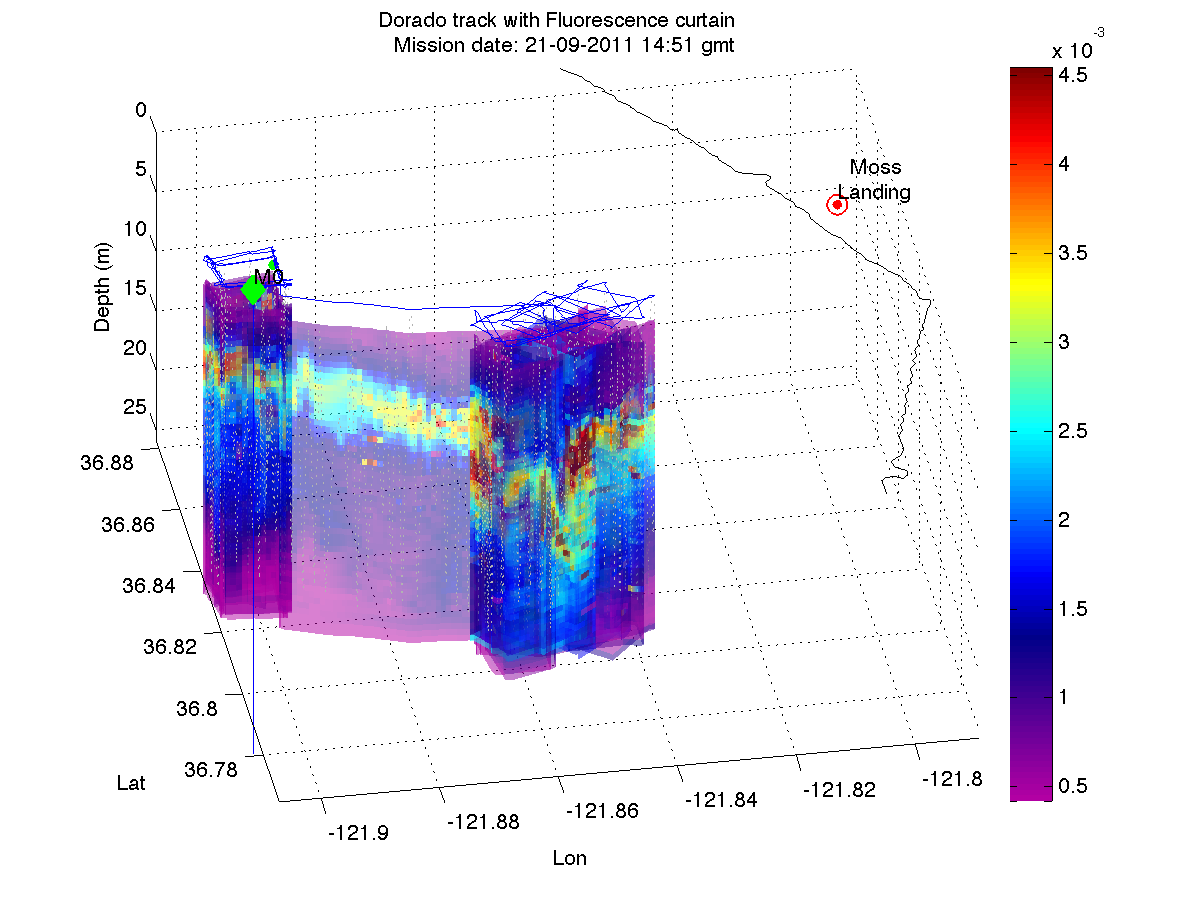
\includegraphics[width=0.5\textwidth]{figs/sep11-ww-flh.png}} 
\subfloat[Nitrate]{\label{fig:sep11-n2}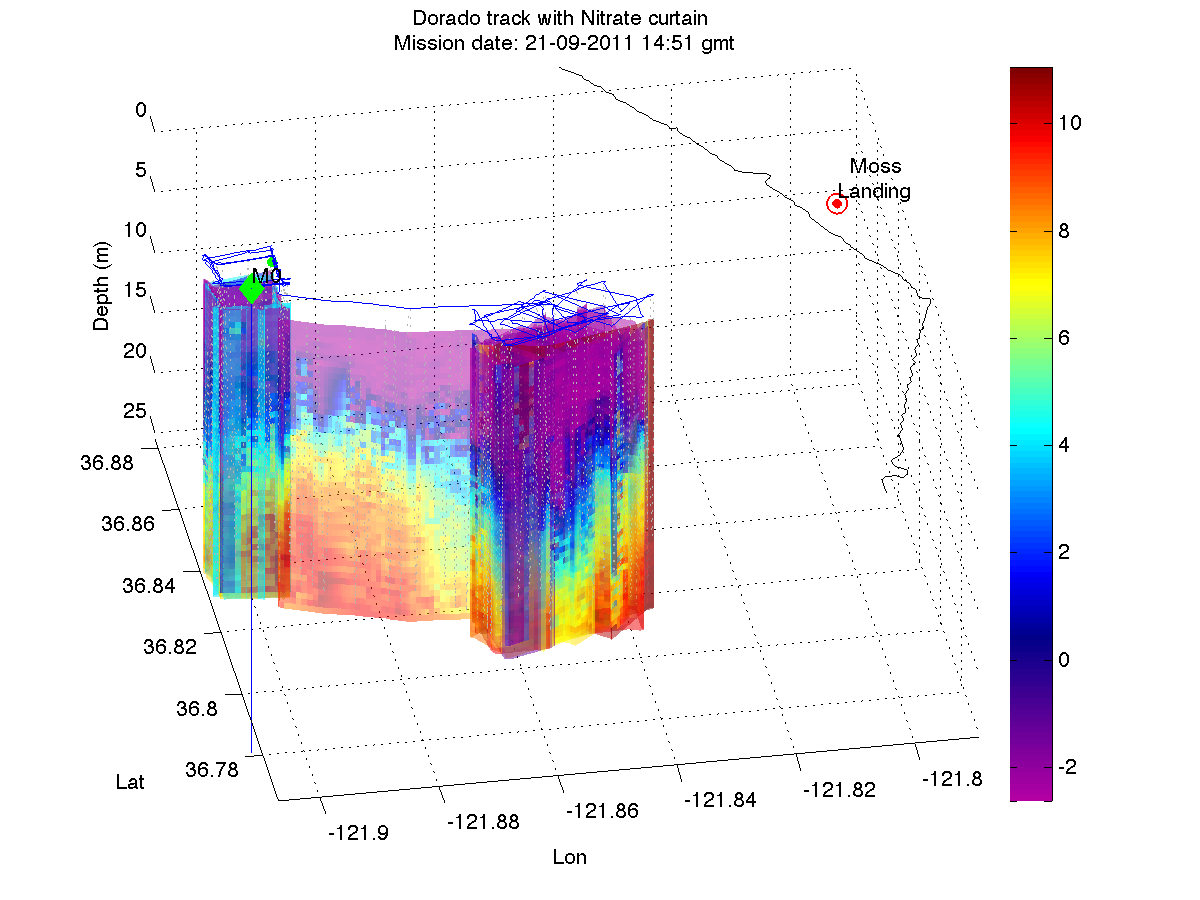
\includegraphics[width=0.5\textwidth]{figs/sep11-ww-n2.png}} 
\caption{\small Interpolated results of a September 2011 \rx mission
  in the Monterey Bay with the profiling \texttt{Wirewalker}
  \cite{rainville01,pinkel11} instrument. Plots show the instrument
  was entrained between two fronts. \emph{Image courtesy: Rishi
    Graham, MBARI}}
  \label{fig:sept11-wirewalker}
\end{figure*}

More interesting experiments are being carried out as a basis to track
more dynamic features such as ocean fronts \cite{fronts11} and
tracking more capable drifting platforms. In particular experiments
with a profiling CTD instrument, the \texttt{Wirewalker}
\cite{rainville01,pinkel11} are resulting in new modalities of making
Lagrangian and Eulerian observations. Fig. \ref{sep11-wirewalker}
shows one such experiment in September 2011 with a GPS-enabled
\texttt{Wirewalker} was tracked by the Dorado running \rx. We are
currently investigating spatio-temporal correlations \cite{gneiting07}
of CTD data obtained by the \texttt{Wirewalker} and tying it to the
observations made in the contextual environment by the Dorado's
sensors.
